\begin{textblock}{9.5}(0., -4.)
    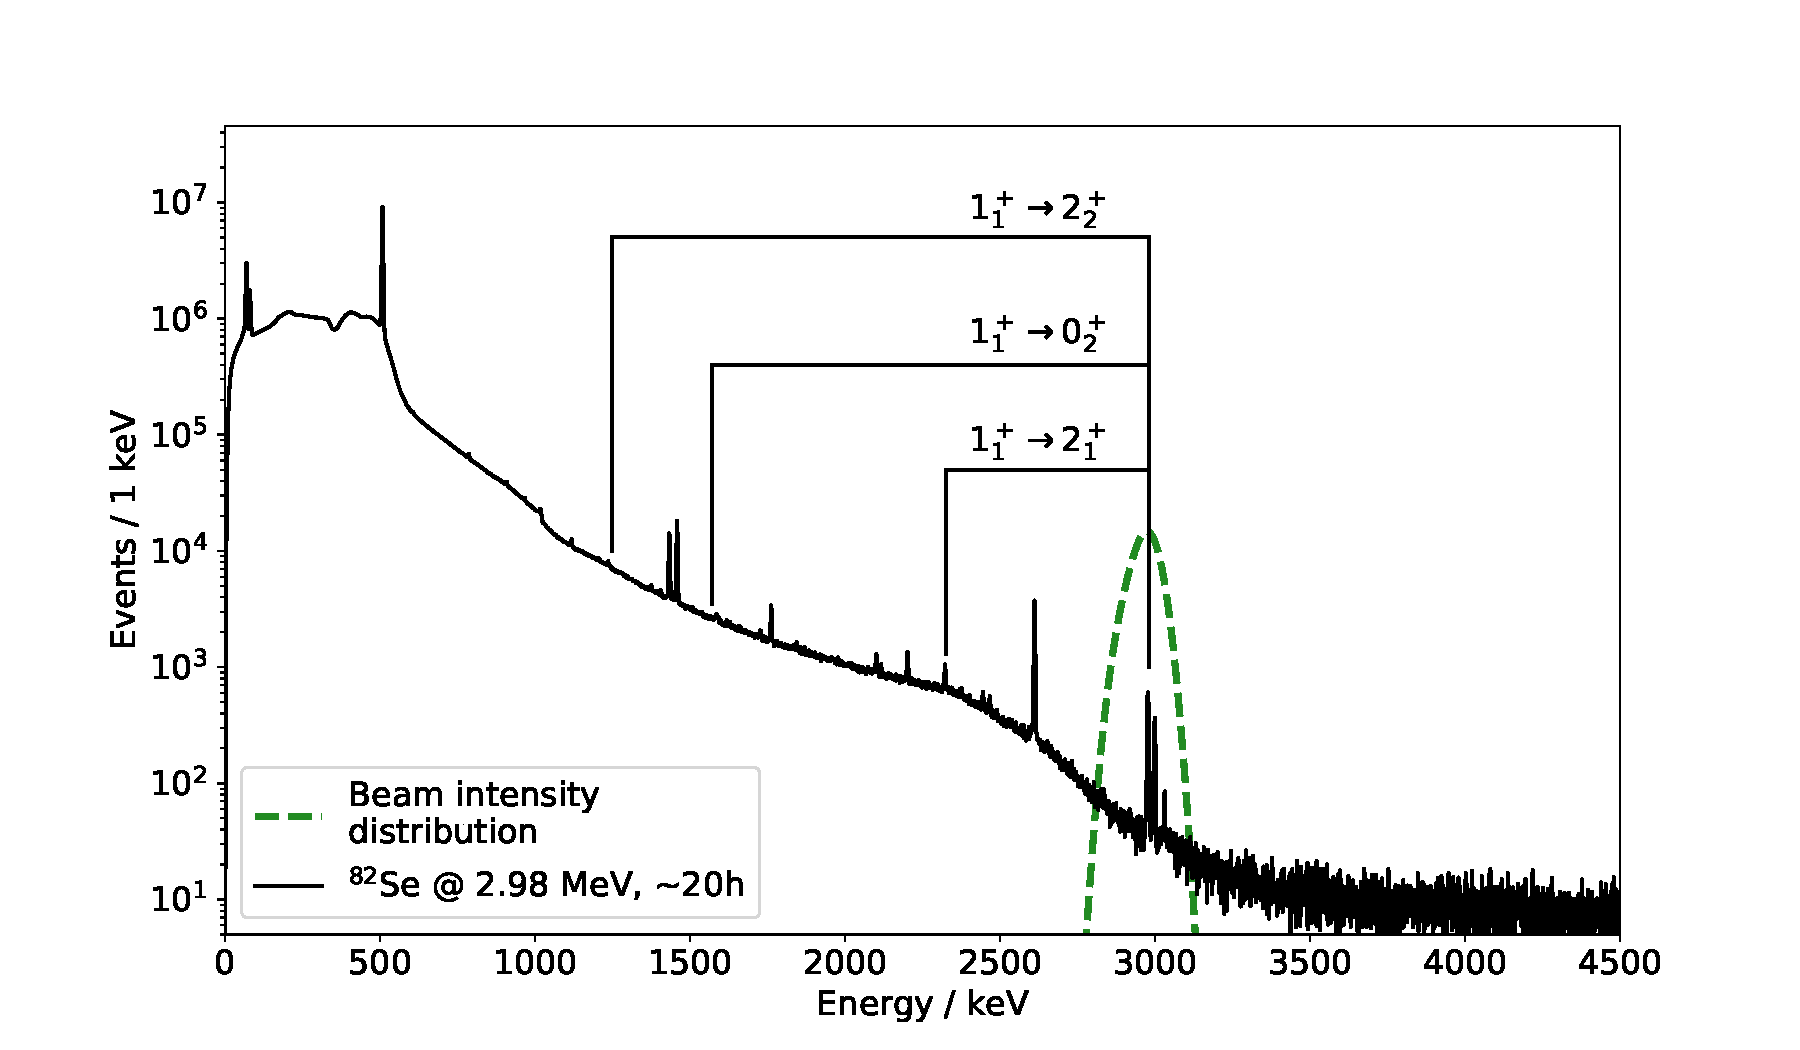
\includegraphics[width=\textwidth, trim=50 0 50 50,clip]{figures/se82_spectrum_branchings.pdf}
\end{textblock}

\begin{textblock}{5.}(10., -5)
    \color{green}\textbf{Advantages} \color{black} of the NRF technique
    \begin{itemize}
        \item Model-independent
        \item High resolution
        \item (Selectivity)
    \end{itemize}
    
    \color{red}\textbf{Disadvantages}\color{black}
    \begin{itemize}
        \item Nonresonant background
        \item Low cross section (long experiments, large samples, stable isotopes)
        \item Inefficient detection
    \end{itemize}
\end{textblock}